% ********** Related work **********

\chapter{Related work}

There are many Medium Access Control (MAC) protocols that cover a multitude of
applications and scenarios. It is a broad research area, and recently there
has been much work done in the area of low-power protocols and wireless networks. MAC
protocols designed for Wireless Sensor Networks can be broadly divided in two
categories: contention-based and TDMA-based protocols.

Contention-based MACs, such as the IEEE 802.11 Distributed Coordination
Function\cite{ieee1997wireless} (DCF), are used in ad-hoc wireless networks.
These protocols do not involve any synchronization between the nodes of the
network. They do however tend to have higher energy consumption because of idle
listening.

TDMA-based protocols require scheduling and the reservation of communication
slots. This is why they present a natural energy conservation advantage over
contention-based protocols as sleep periods can be increased and there is no
overhead caused by contention or collisions.

\section{S-MAC}

S-MAC\cite{ye2004medium} is a Medium Access Control protocol that attempts to
reduce power consumption by reducing collisions, overhearing, control overhead
and idle listening. It also aims to offer good scalability and collision
avoidance. It uses Request to Send/Clear to Send (RTS, CTS) signals in order to
reduce collisions and alternating listen/sleep periods to reduce energy
consumption. However, these improvements come at the price of latency. 

In order to reduce control overhead, neighbouring nodes are synchronized.
However, not all neighbouring nodes can be on the same schedule.  Figure
\ref{fig:s-mac_schedules} presents and example of two nodes, A and B, that
synchronize with nodes C, respectively D, which are on different
schedules. This means they must use the RTS/CTS signals to avoid causing a
collision. After nodes start a data transmission, they do not go back to sleep
until it has ended.

\begin{figure}[ht]
	\begin{center}
		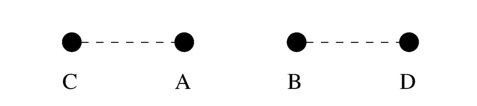
\includegraphics{img/s-mac_schedules.pdf}
	\end{center}
	\caption{\small \itshape{Neighbouring nodes A and B with different
	schedules\protect\footnotemark}}
	\label{fig:s-mac_schedules}
\end{figure}
\footnotetext{Image taken from \emph{Medium access control with coordinated
adaptive sleeping for wireless sensor networks}\cite{ye2004medium}}

Synchronization between nodes is achieved by maintaining a schedule table that
stores the schedules of all known neighbours. At startup, a node listens for a
schedule advertised by other nodes before choosing its own, randomly. If it
receives a schedule before choosing its own, it follows that schedule. If
however a schedule arrives after it has chosen its own, it adopts both schedules
but advertises only its own.

Timer synchronization, in order to prevent clock drift, is
accomplished with special SYNC packets.

\section{SCP}

Scheduled Channel Polling\cite{ye2006ultra} (SCP) is another MAC protocol which
is based on S-MAC. The main problem it addresses is long preambles added to
packets. Nodes function on cyclic schedules of sleeping and listening. If a
node does not detect a transmission during the listening period it goes back to
sleep, otherwise it remains active to receive the transmission. This means that
a node that wants to send a message must first send a preamble signal during
the destination node's listening period. Because of clock drift this preamble
can become quite long, especially in the case of long synchronization periods,
as shown in figure \ref{fig:scp_long_preambles}.

SCP addresses this problem by maintaining a schedule for listening periods.
This means that a node can anticipate when the destination node will be
listening and can greatly reduce the preamble length, as shown in figure
\ref{fig:scp_short_preambles}.

Although scheduling does reduce preamble length it also adds synchronization
overhead. This can be solved by adding synchronization information to data
packets, however that is not always possible. In the case that there is no data
packet to which to append the synchronization information a separate
\emph{sync} packet will be sent.

\clearpage

\begin{figure}[ht]
	\begin{center}
		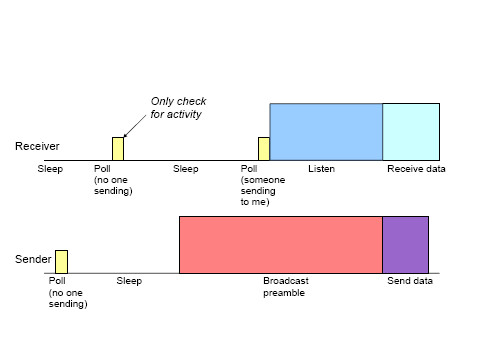
\includegraphics[scale=0.9]{img/scp_long_preambles.jpg}
	\end{center}
	\caption{\small \itshape{Long preamble needed without
	scheduling\protect\footnotemark}}
	\label{fig:scp_long_preambles}
\end{figure}
\footnotetext{Image taken from \emph{Ultra-low duty cycle MAC with scheduled
channel polling}\cite{ye2006ultra}}

\begin{figure}[ht]
	\begin{center}
		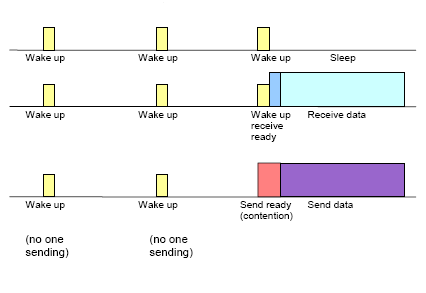
\includegraphics[scale=0.9]{img/scp_short_preambles.jpg}
	\end{center}
	\caption{\small \itshape{Short preamble needed when using scheduled 
	listening\protect\footnotemark}}
	\label{fig:scp_short_preambles}
\end{figure}
\footnotetext{Image taken from \emph{Ultra-low duty cycle MAC with scheduled
channel polling}\cite{ye2006ultra}}

% ********** End of Related work **********
